\chapter{Kinematic Constraints}
\label{Constraints}

\section{Introduction}

Most of complex mechanical systems contains kinematic constraints.
There are many different types of them. The constraints that affect
the motion of a car-like robot are an important example of
nonholonomic kinematic constraints.

Kinematic constraints to be handled are a particular case of holonomic
constraints.  Normally, this type of constraints make the mechanical
system to loose some of its degrees-of-freedom (d.o.f.). In our case,
the value of the lost d.o.f. are calculated from the values of some of
the others d.o.f. of the system. So joints of the mechanical system
can be divided into two types: active and passive. Active joints
represent the real d.o.f. of the mechanical system. Passive joints are
controlled by active ones, so they are not really d.o.f. Closed
kinematic chains are the most interesting and complicated particular
case of this type of constraints.


\section{Method}

The method used in Move3D in order to obtain motion paths for
mechanical systems containing the above mentioned type of kinematic
constraints is based on a geometrical solution.

First of all, the geometric constraint
equation(s) associated with the involved joints of the system have to
be calculated. Once we have this(these) equation(s) we will
be able to plan for the constrained mechanical system within
Move3D. Nodes of the roadmap are generated by sampling random
configurations that ignore kinematic constraints. The way to get
constrained configurations by this method consist of applying the constraint
equations to the random configuration. By means of these equations,
the value of the passive joints affected by the constraint are changed
and they are induced to be in agreement with it. The edges of the roadmap are
generated in a similar way. The local planner generates the
configurations of the local path between two nodes. Along this path,
the geometric constraint equations are applied to each one of these
intermediate configurations in order to update the value of the
constrained (passive) joints.

Therefore, with this methodology, any kinematic constraint
representable as one or several equations relating the joints of the
system will be able to be handled by Move3D.


\section{Treated constraints}

The already included  kinematic constraints in the Move3D 
are:

\begin{itemize}
\item Linear relationship between two d.o.f..
\item $RRPR$, $4R$ and $3RPR$ linkages.
\item Contact with ground.
\item Car front wheels.
\item Planar closed chain.
\end{itemize}

Next, each one of the above listed constraints will be explained.  The
treatment of some other more complicated cases remains as a future
work.


\subsection*{Linear relationship between two d.o.f.}

The first kinematic constraint included in Move3D is
simple but quite useful. It consist in impose a linear relationship
between two of the d.o.f. of the robot. There are an active and a
passive joints. The passive joint $JA$ is updated to the value of the
active one $JB$ multiplied by a constant $K$. A possible offset $C$
has been also considered. So the geometric constraint equation in this
case is:
\[JA = K \cdot JB + C\]


Lots of different examples of mechanical system containing this simple 
kinematic constraint could be found. For instance, actuators doing 
the same movement is a typical case of two d.o.f. keeping a linear
relationship. Figure~\ref{fig:halteres} shows an example of this
case. There, two robots are cooperating in a task. Each robot is
equipped with a hydraulic bar. These bars must have the same
displacement in the two robots in order to obtain a nice
comportment.


\begin{figure}[ht!]
\centerline{
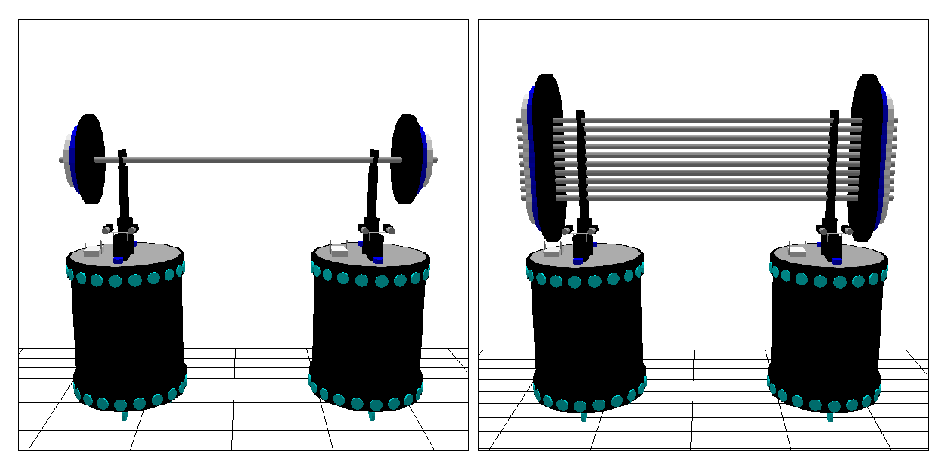
\includegraphics[width=10cm]{FIG/Constraint/halteres.eps}
}
\centerline{
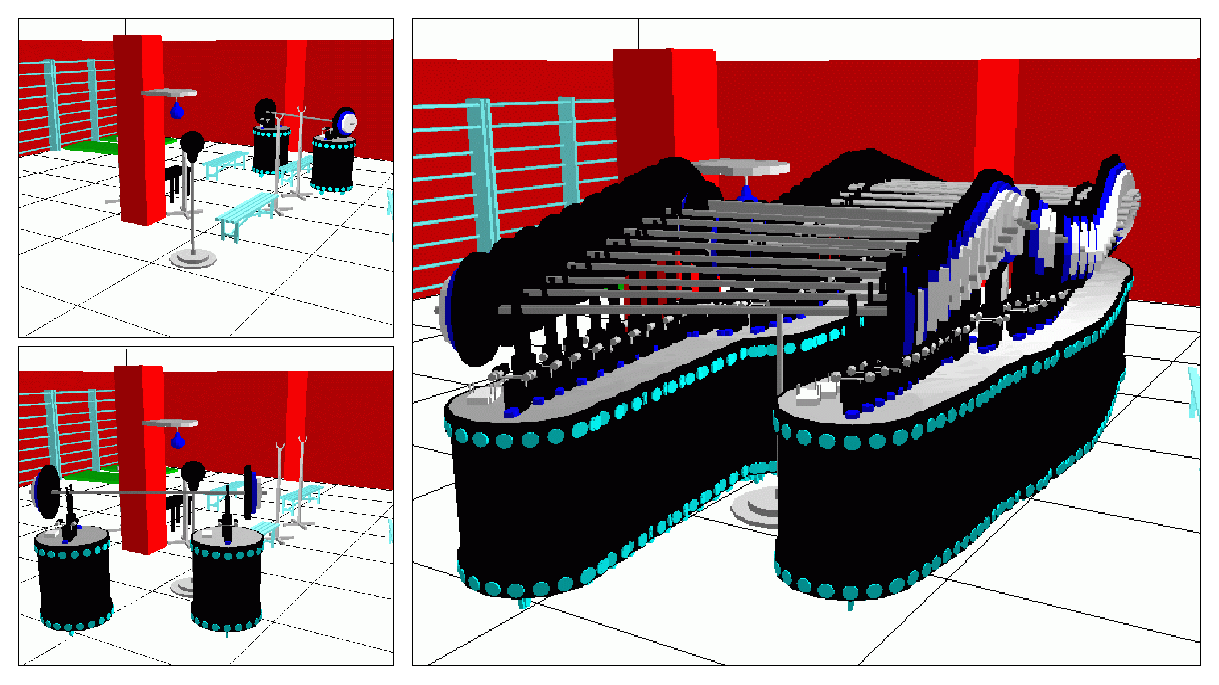
\includegraphics[width=10cm]{FIG/Constraint/halteres2.eps}
}
\caption{\label{fig:halteres} Two holonomic robots cooperating in a
task. The bar with the weighs must stay horizontal, so the hydraulic
bars of the robots must move at the same time.}
\end{figure}


Another example of application of this kinematic constraint would be
the incorporation of natural effects in the simulating model. The
constraint represented in Figure~\ref{fig:dedos} corresponds to the
natural motion of a finger. There is a relationship between the
movement of the phalanges of a hand finger. It could be modeled in a
simple way as a linear relationship.

\begin{figure}[ht!]
%\vspace{15.0mm}
\begin{center}
  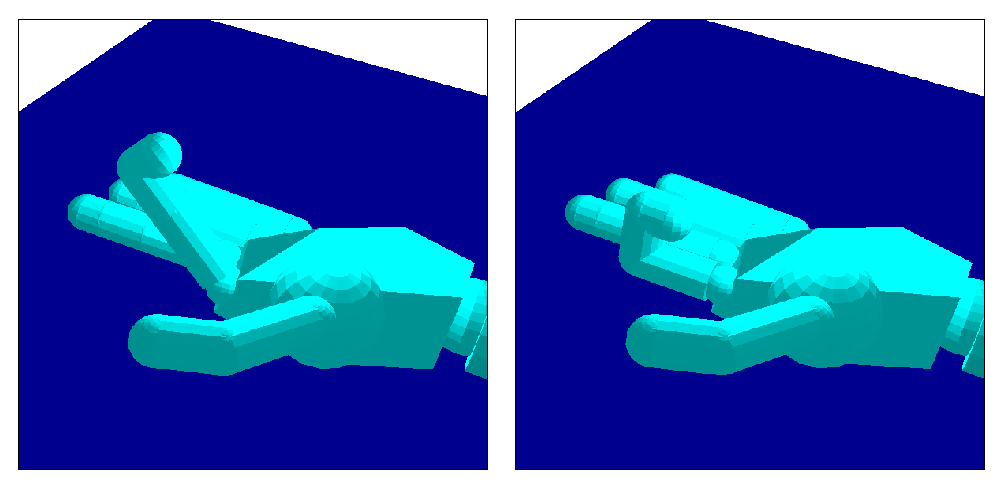
\includegraphics[width=10.0cm]{FIG/Constraint/dedos.eps}
\end{center}
\caption{\label{fig:dedos} Constraint in the movement of a finger. The 
left figure shows an abnormal position for a finger, the right one shows a 
normal situation.}
%\vspace{5.0mm}
\end{figure}


\subsection*{$RRPR$, $4R$ and $3RPR$ linkages}

The $RRPR$, $4R$ nd $3RPR$ linkages are basic planar closed kinematic
chains. Theirs constraint equations are calculated by planar geometry,
likewise theirs motion limits. It must be remarked that {\bf joints
  affected by these constraints must be defined on the same plane}.
Next each one of these linkages will be separately explained.

%\vspace{5.0mm}
\begin{figure}[ht!]
%\vspace{5.0mm}
\begin{center}
\psfrag{teta}[l]{$\theta$} 
\psfrag{chi}[l]{$\psi$}
\psfrag{r}[l]{$r$}
\psfrag{s}[l]{$s$}
\psfrag{g}[l]{$g$}
\psfrag{e}[l]{$e$}
  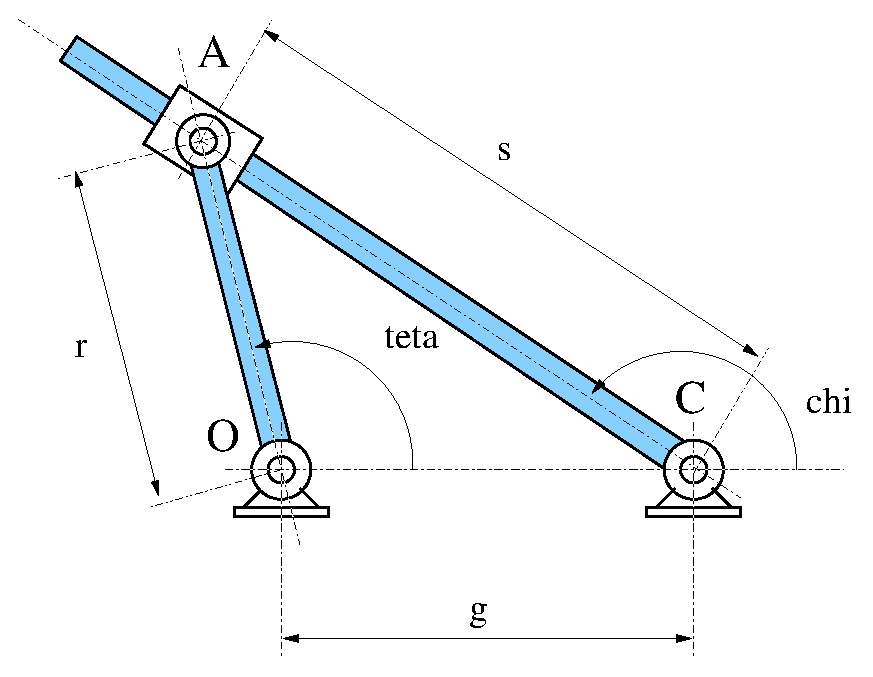
\includegraphics[width=7.0cm]{FIG/Constraint/RRPR2.eps}
\end{center}
\caption{\label{fig:RRPR} The dimensions characterizing an $RRPR$
linkage.}
%\vspace{5.0mm}
\end{figure}


The $RRPR$ linkage is known as a {\em slider-crank} and consist of two
rotating cranks linked by a translating slider. It is a one
degree-of-freedom planar closed chain that is a fundamental machine
element found in everything from automotive engines to door closing
mechanisms.

In the implementation of this constraint in Move3D, the
translation $s$ has been chosen to be the d.o.f. that controls the chain. Therefore,
the joint representing $s$ ($JA$) will be the active joint and the joints
representing $\theta$ ($JO$) and $\psi$ ($JC$) will be the passive
ones. Notice that $JO$ and $JC$ must have the same parent, and $JA$
must be placed in the point corresponding to {\bf A} in the modeling.

\begin{figure}[ht!]
\begin{center}
\psfrag{teta}[l]{$\theta$} 
\psfrag{chi}[l]{$\psi$}
\psfrag{fi}[l]{$\phi$}
\psfrag{a}[l]{$a$}
\psfrag{h}[l]{$h$}
\psfrag{g}[l]{$g$}
\psfrag{b}[l]{$b$}
 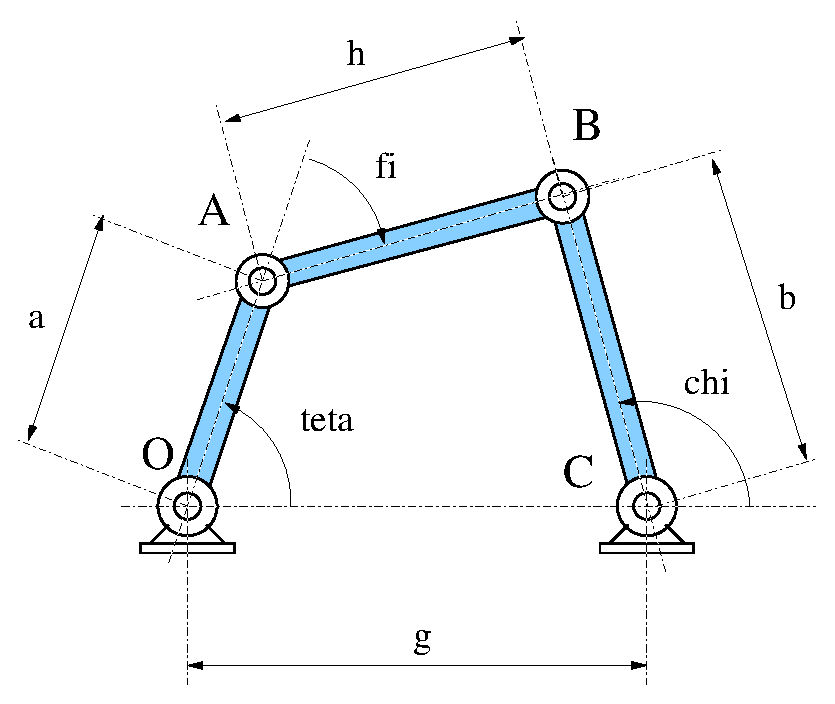
\includegraphics[width=7.0cm]{FIG/Constraint/4R.eps}
\end{center}
\caption{\label{fig:4R} The dimensions characterizing an $4R$ linkage.}
\end{figure}

The $4R$ linkage is a four-rotations planar closed chain. It consist
of an input crank ({\bf OA}), an output crank ({\bf CB}) and a coupler 
({\bf AB}). There is also just one d.o.f. in this fundamental mechanism,
which is the input crank.  

The following remarks must be obeyed for the modeling of this chain:
$JO$ and $JC$ must be defined on the same solid; the coupler must be
defined from the input crank, that is, the chain is cut at {\bf B};
the joint $JB$ can be placed at the end of the output crank or at the
end of the coupler, but this joint is necessary in order to calculate
lengths of the links.

The $3RPR$ linkage can be seen as a $4R$ linkage where the length of
the output crank is variable. It is, therefore, a two d.o.f. planar
closed chain. These two active joints corresponds to the input crank
({\bf OA}) and the translating slider placed at {\bf B} on the output
crank. 

\begin{figure}[ht!]
\begin{center}
\psfrag{teta}[l]{$\theta$} 
\psfrag{chi}[l]{$\psi$}
\psfrag{fi}[l]{$\phi$}
\psfrag{a}[l]{$a$}
\psfrag{h}[l]{$h$}
\psfrag{g}[l]{$g$}
\psfrag{s}[l]{$s$}
 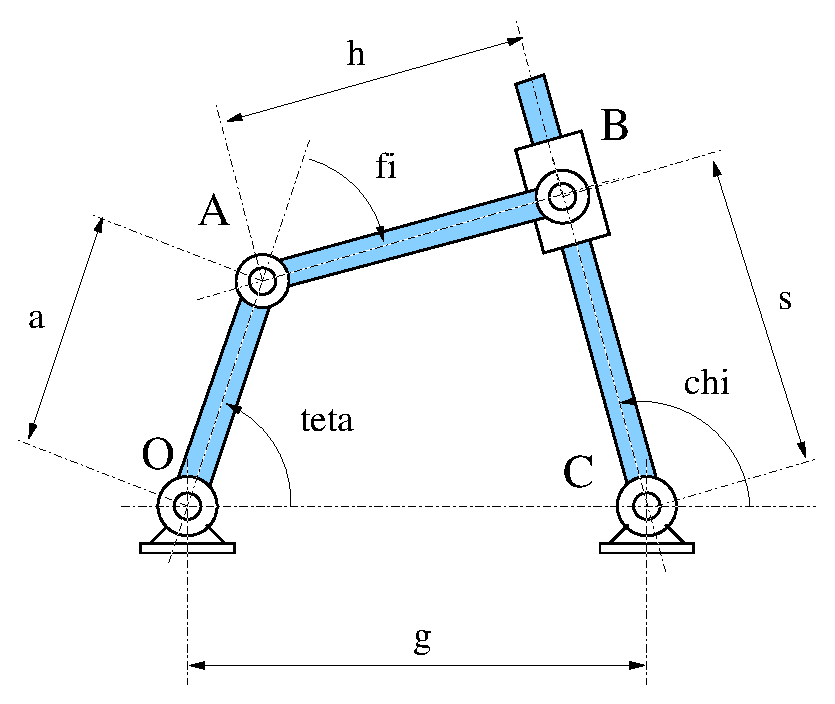
\includegraphics[width=7.0cm]{FIG/Constraint/3RPR.eps}
\end{center}
\caption{\label{fig:3RPR} The dimensions characterizing an $3RPR$ linkage.}
\end{figure}

The remarks for the modeling are similar to the ones made for the
$4R$ linkage, but in this case $JB$ is the translating joint, and it
must be defined from the output crank.

Now, some of the results obtained before the
implementation of these constraints in Move3D will be shown. Figures~\ref{fig:excavator}
represents the model of an hydraulic excavator. The motion of its arm
is controlled by the hydraulic systems, so there are 3 d.o.f.. This
mechanical system contains four closed kinematic chains. Three of them
are the hydraulic systems, and the fourth one is the mechanism for the
motion of the bucket. The hydraulic systems can be modeled as $RRPR$
linkages where the translating crank is the hydraulic bar. The
mechanism of the bucket is a $4R$ linkage. But the third hydraulic
system and the mechanism of the bucket are linked, so we really have
two single closed chains and one double loop closed chain.

\begin{figure}[hb!]
\begin{center}
  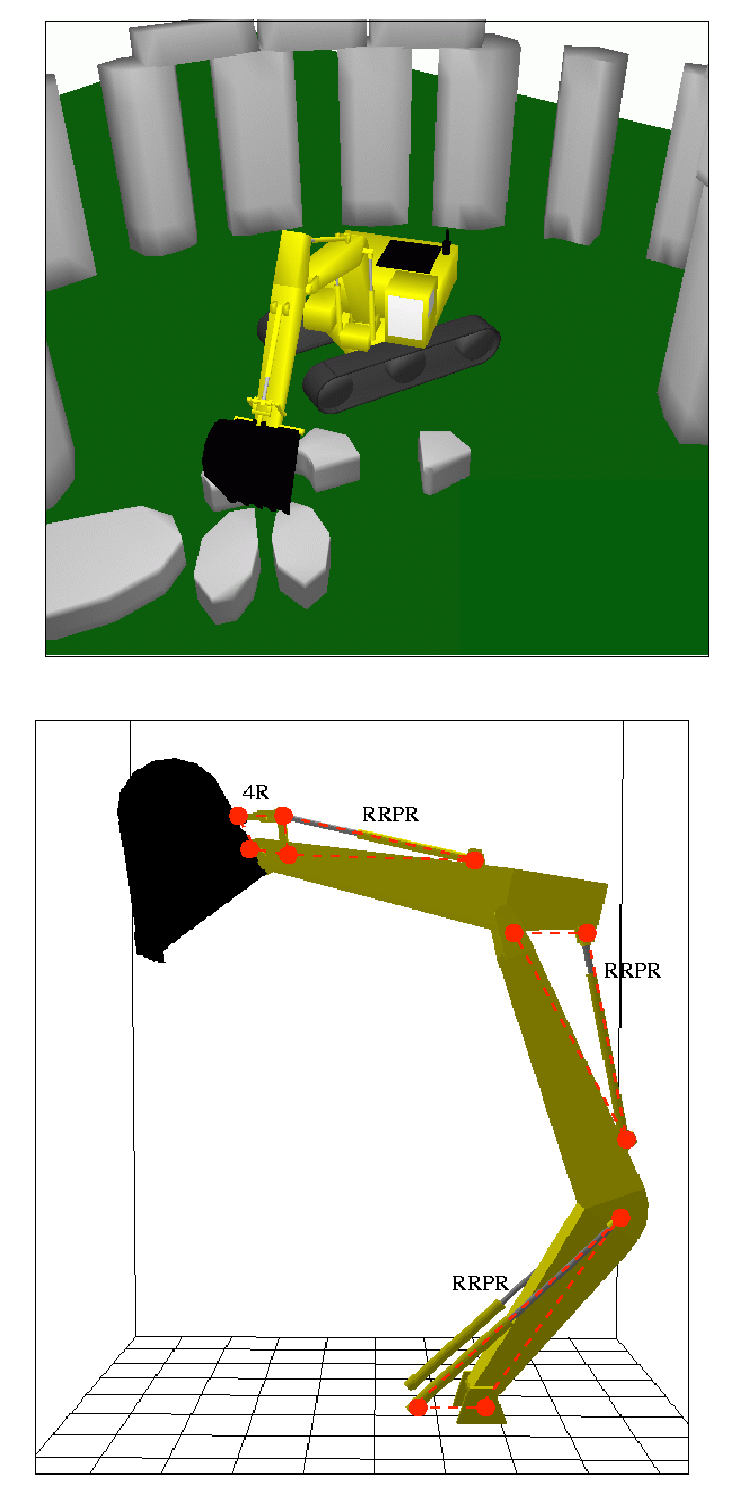
\includegraphics[width=8.1cm]{FIG/Constraint/excavator.eps}
\end{center}
\caption{\label{fig:excavator} Hydraulic excavator. This model
contains two single closed chains and one double loop closed chain. The 
arm, a mechanical system of 19 d.o.f. has been constrained to a system of 3 d.o.f..}
\end{figure}


\begin{figure}[ht!]
\begin{center}
  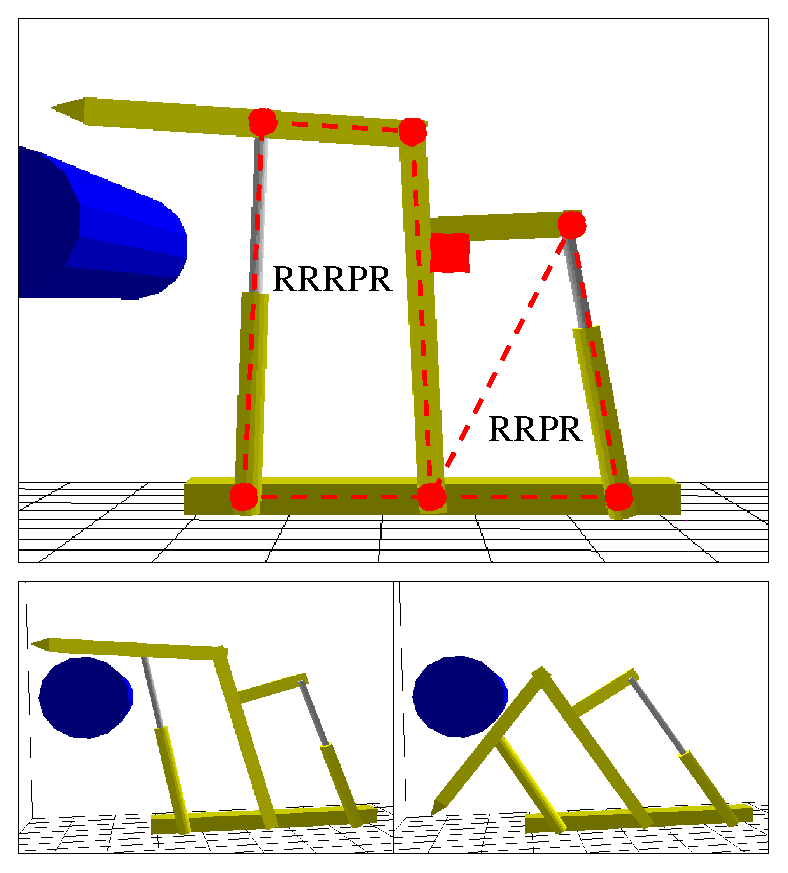
\includegraphics[width=8.0cm]{FIG/Constraint/liegeois.eps}
\end{center}
\caption{\label{fig:liegeois} Manipulator shown in some works of Liegeois.
This two d.o.f. mechanical system consist of a double loop closed chain.} 
\end{figure}

The mechanical system in Figures~\ref{fig:liegeois} is another example
of a double loop closed chain. In this case, the two single chains are 
a $RRPR$ linkage for the rear hydraulic system, and a $3RPR$ linkage
for the front loop.


\subsection*{Contact with ground}

This kinematic constraint represents the case when an object is
required to stay in contact with an obstacle. Particularly, the
implemented constraint corresponds to an object that have to move with
its lowest point sliding on the ground.

The kind of problems which we are mainly interested in are mobile
machines (robots) carrying long objects that have to trail on the
ground. However, the general problem has not been already solved. Just
the last joint of the robot, that is, the joint of the terminal organ
of the robot which grasp the carried object, is going to be
controlled.  This joint must be a revolute joint turning around an
axis perpendicular to the absolute $z$-axis of the scene. This
particular case can be seen as a planar problem.

\begin{figure}[ht!]
\begin{center}
\psfrag{te}[l]{$\theta$} 
\psfrag{li}[l]{$\theta_{JC}$}
\psfrag{de}[l]{$\theta o_{JC}$}
\psfrag{ang}[l]{$\theta_{Object}$}
\psfrag{ant}[l]{$\theta_P$}
\psfrag{d}[l]{$d$}
\psfrag{z_J}[l]{$z_J$} 
\psfrag{z_G}[l]{$z_0$}    
  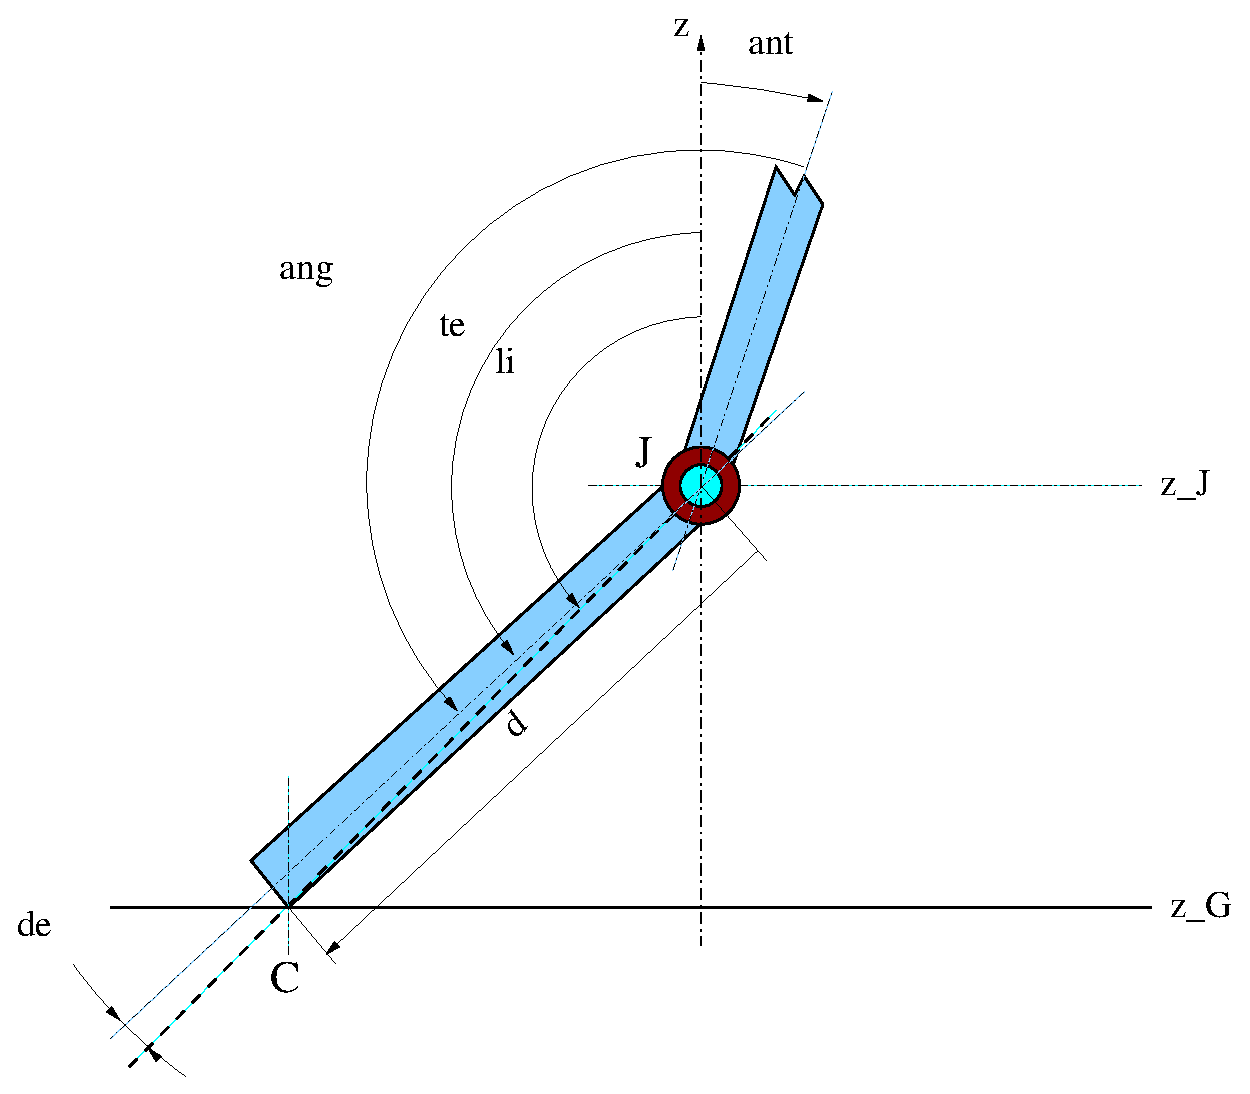
\includegraphics[width=7cm]{FIG/Constraint/ground.eps}
\end{center}
\caption{\label{fig:ground} Variables and references in the analysis.}
\end{figure}

Some remarks for the modeling must be made for this constraint. Let us 
suppose that, for long-shaped objects, the point having to stay
in contact with the ground does not change. In the file containing the
workspace for the path planning with Move3D, the carried object must
be modeled as another body of the robot. Therefore, a joint can be
placed in the point of this `body' that has to slide on the ground.
This joint will be or not a connection with another body, so it will
be not a real joint, but it is necessary to include it in the model.
Let us call it {\bf $J_C$} because it is placed at the point {\bf C}.
It must not be forgotten during the modeling that we are solving a
planar problem. That is to say that the points {\bf J} and {\bf $J_C$}
must be in the same plane, and this plane must be perpendicular to the
rotation axis of the joint at {\bf J}.

\begin{figure}[ht!]
\begin{center}
  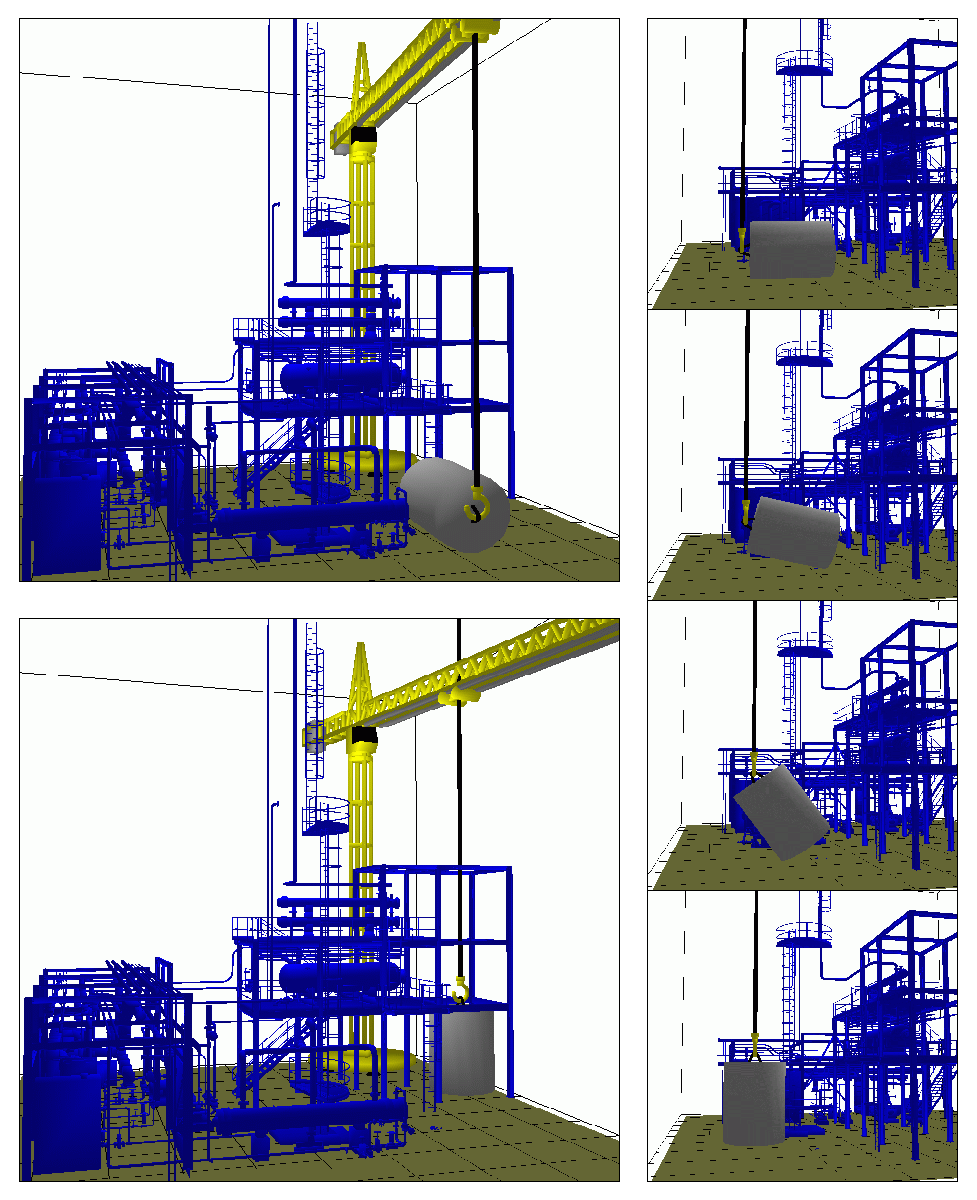
\includegraphics[width=8.0cm]{FIG/Constraint/grue.eps}
\end{center}
\caption{\label{fig:gruaind} A crane has to place a tank into a
metallic structure in an industrial environment. In the initial
configuration, the tank is horizontally placed on the ground. The tank
has to slide on the ground before it reaches the vertical position.}
\end{figure}

Applications of this kind of kinematic constraint are particularly
interesting. For instance, in industrial environments they exist path
planning problems where a moving object must stay in contact with the
ground following physical laws. Figure~\ref{fig:gruaind} shows an
example of one of these problems. The typical example of application,
also usual in the industrial environments, consist in a `robot'
carrying long-shaped objects with a point sliding on the ground. The
example in Figure~\ref{fig:pipe} shows the performance of the planner
handling this kind of kinematic constraint.

\begin{figure}[ht!]
\centerline{
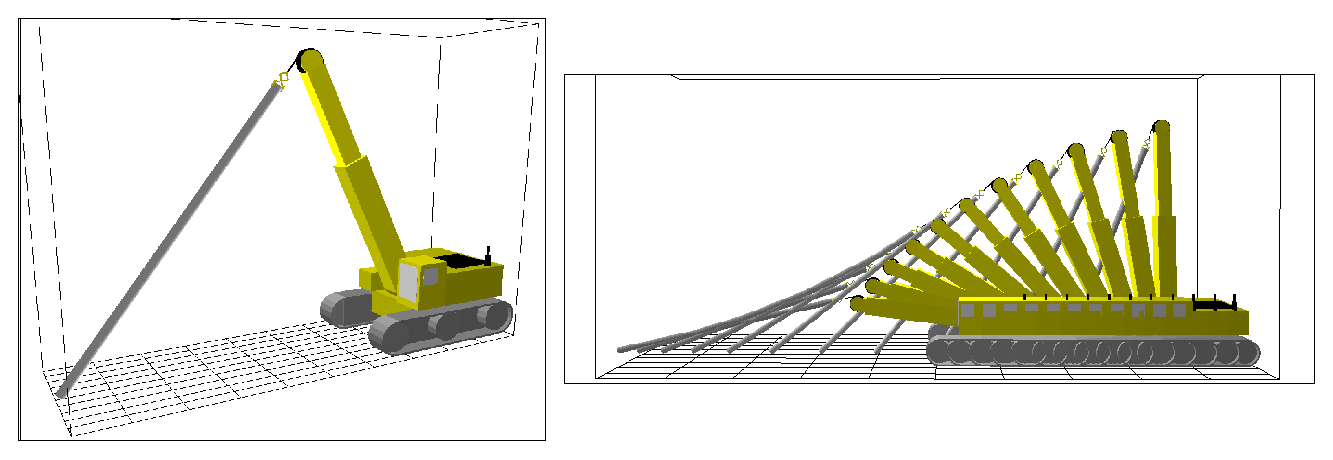
\includegraphics[width=15cm]{FIG/Constraint/pipe12.eps}
}
\caption{\label{fig:pipe} A telescopic handler carries a long
pipe. The lowest extreme of the pipe must stay in contact with the
ground all along the path.}
\end{figure}

\subsection*{Car front wheels}

\begin{figure}[ht!]
\begin{center}
\psfrag{t}[l]{$\theta$} 
\psfrag{O}[l]{O} 
\psfrag{P}[l]{P}    
  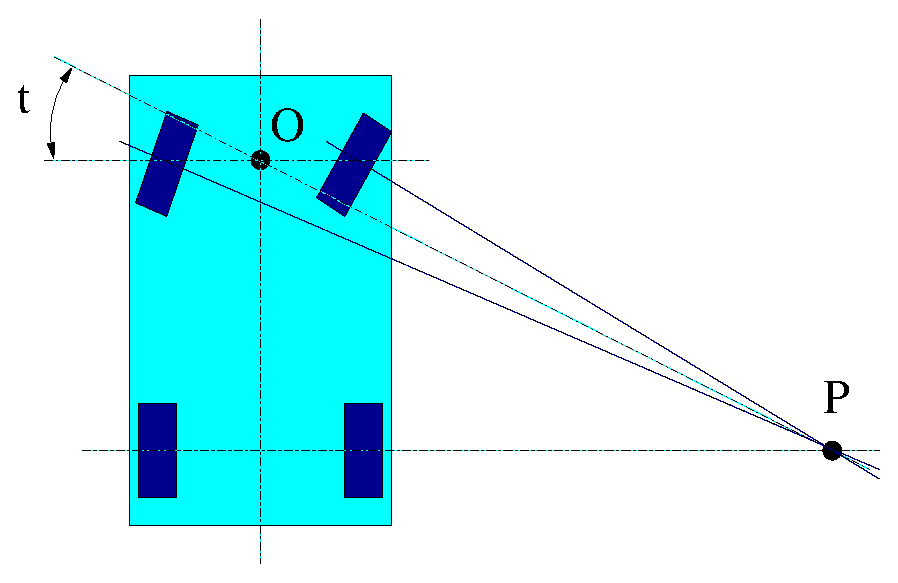
\includegraphics[width=8cm]{FIG/Constraint/carfw.eps}
\end{center}
\caption{\label{fig:carfw} Geometric law for the angles of the car 
  front wheels.}
\end{figure}

This kinematic constraint will be applied to cars. A car can be
modeled as a robot towing a trailer. The steering column of the car is
represented by the robot and the body of the car is represented by the
trailer (see Chapter~\ref{methode-local}). The angle of each
front wheel is then computed as shown on Figure~\ref{fig:carfw}.
That is, the axes of all the wheels (front and rear) must coincide in
a same point {\bf P}.  This point is also the intersection between the
rear wheels axis and the line passing trough the car turning center
(steering column) {\bf O} and having the car turning angle $\theta$.
This point {\bf O} represents the joint between the robot and the
trailer.

Figure~\ref{fig:LegoCar} shows the model of a car
within this constraint has been successfully tried.



\begin{figure}[htb!]
\begin{center}
  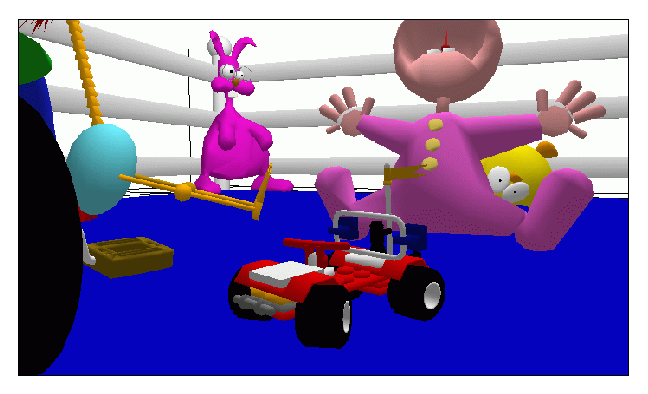
\includegraphics[width=8cm]{FIG/Constraint/LegoCar.eps}
\end{center}
\caption{\label{fig:LegoCar} Three-dimensional model of a LegoCar.}
\end{figure}


\subsection*{Planar closed chain}

A general analytical solution for a planar closed
chain is used in this constraint. It is known that for a n-bar planar mechanism, the number of
d.o.f is n-3. The base of the mechanical system is considered as one
of the bars, then it becomes a (n-1)-bar mechanism with (n-1)-2 d.o.f.
The chosen method to solve this geometrical problem
consist of cutting the loop in two parts. At one side we leave a 2-bar
open chain. At the other side we will have another open chain with the
rest of the elements. The two joints of the first part will be the
passive joints (the two lost d.o.f.), while the joints the other part
remain active. The angles of the passive joints are calculated by
trigonometric laws in order to close the loop.

\begin{figure}[h!]
\begin{center}
\psfrag{a}[l]{$\theta 1$} 
\psfrag{b}[l]{$\theta 2$}
\psfrag{chi}[l]{$\psi$}
\psfrag{fi}[l]{$\phi$}
\psfrag{d}[l]{$d$}
\psfrag{any planar open chain}[l]{any planar open chain}
  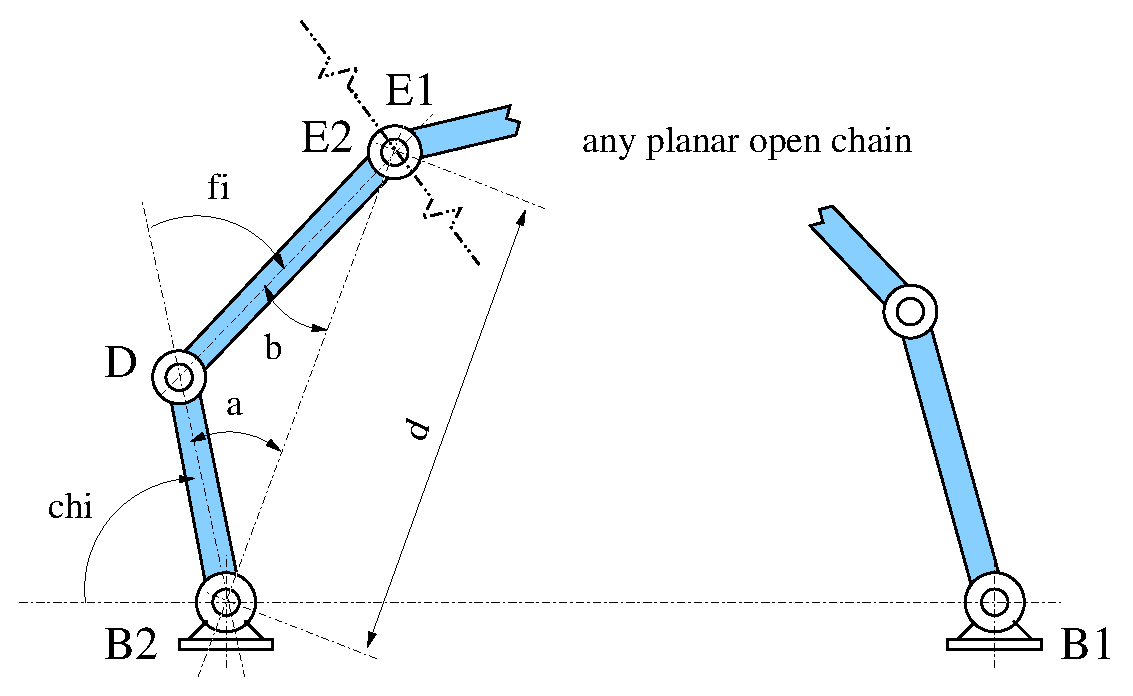
\includegraphics[width=7cm]{FIG/Constraint/plclch.eps}
\end{center}
\caption{\label{fig:plclch} Variables and references in the analysis.}
\end{figure}

Figure~\ref{fig:plclch} represents the way how a mechanical system 
containing this kinematic constraint must be modeled. Joints ({\bf E1}
and {\bf E2}) must be placed at the end of each open chain.

Figure~\ref{fig:cad8pas} shows the performance of Move3D solving a 
path planning problem for a 8-bar closed chain.

\begin{figure}[h!]
\begin{center}
  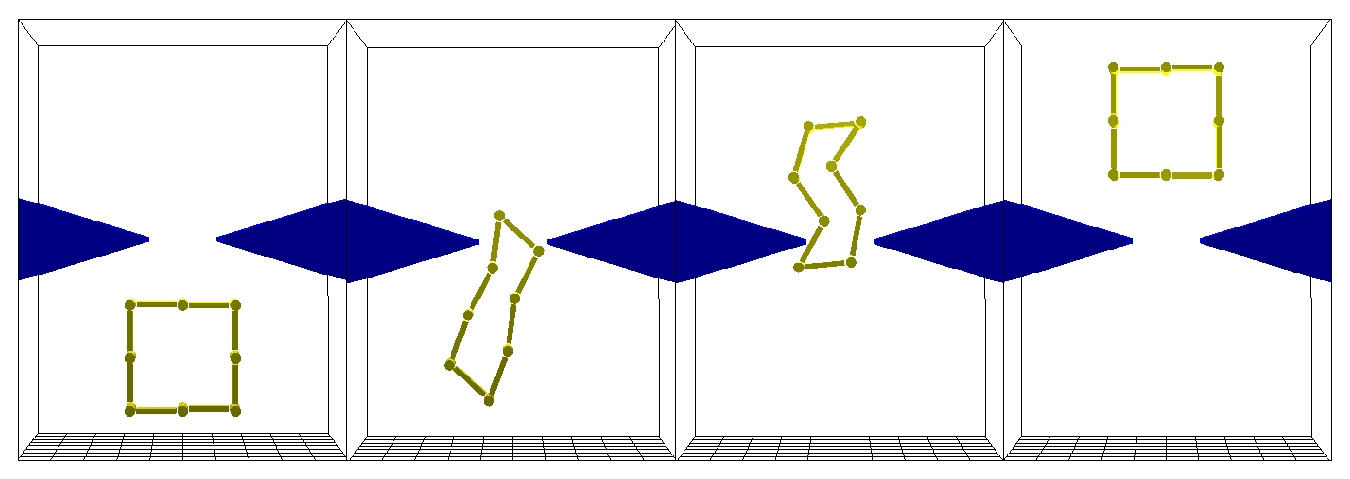
\includegraphics[width=10cm]{FIG/Constraint/cad8pas.eps}
\end{center}
\caption{\label{fig:cad8pas} Some sequences of the solution given
  by Move3D for a 8-bar closed chain that has to find a path trough a
  narrow passage.}
\end{figure}

\section{How to use them}

Kinematic constraints can be set in the mechanical system in two ways: 
they can be directly set in the model input file ({\tt .p3d}), or they can
be set once Move3D is running. Next, this two
possibilities are explained.

\subsection*{Kinematic constraints in the {\tt .p3d} file}

Constraints can be introduced in the mechanical system by adding command 
lines at the end of the model input file. These command lines have the 
following structure: 

\hspace{-4.0mm}
{\tt p3d\_constraint \footnotesize cntrt\_name npasjnts \{pj1...pjn\} nactjnts
  \{aj1...ajn\} nc \{c1...cn\} no \{o1...on\}} \index{p3d\_constraint} \\

where:
\begin{tabbing}
>>>\=>>>>>>>>>>>>> \= \kill
\> - {\tt cntrt\_name} \>: is the name of the kinematic constraint to 
  be set.\\
\> - {\tt npasjnts}   \>: is the number of passive joints.\\
\> - {\tt \{pj1...pjn\}}\>: are the indexes corresponding to each one of 
  the passive joints.\\
\> - {\tt nactjnts}   \>: is the number of active joints.\\
\> - {\tt \{aj1...ajn\}}\>: are the indexes corresponding to each one of 
  the active joints.\\
\> - {\tt nc}         \>: is the number of (real) constant parameters.\\
\> - {\tt \{c1...cn\}}  \>: are the constant parameters of the
  constraint.\\
\> - {\tt no}          \>: is the number of other (integer) constant parameters.\\
\> - {\tt \{o1...on\}}   \>: are integer constant parameters of the
  constraint.\\
\end{tabbing}

  
For each one of the kinematic constraints explained in
the last section, the parameters of this command line are as follows
(see figures in last section for the references of points and joints):

\begin{tabbing}
>\=>>\=>>>>>>>>>>>>\=>>>\= \kill
\>{\normalsize \bf Linear relationship between two d.o.f.} \\
\>\>\\
\>\>{\bf \tt cntrt\_name} \>: {\tt p3d\_lin\_rel\_dofs}\\
\>\>{\bf \tt npasjnts} \>: 1\\
\>\>{\bf \tt pj1} \>: index of the joint to be controlled ($JA$)\\
\>\>{\bf \tt nactjnts} \>: 1\\
\>\>{\bf \tt aj1} \>: index of the joint that controls $JA$ ($JB$)\\
\>\>{\bf \tt nc} \>: 2\\
\>\>{\bf \tt c1} \>: linear relationship coefficient ($K$)\\
\>\>{\bf \tt c2} \>: offset ($C$)\\
\>\>{\bf \tt no} \>: 0\\
\>\>\\
\>{\normalsize \bf $RRPR$ linkage} \\
\>\>\\
\>\>{\bf \tt cntrt\_name} \>: {\tt p3d\_RRPRlnk}\\
\>\>{\bf \tt npasjnts} \>: 2\\
\>\>{\bf \tt pj1} \>: index of the joint corresponding to {\bf O}\\
\>\>{\bf \tt pj2} \>: index of the joint corresponding to {\bf C}\\
\>\>{\bf \tt nactjnts} \>: 1\\
\>\>{\bf \tt aj1} \>: index of the translating joint, placed at {\bf A}\\
\>\>{\bf \tt nc} \>: 0\\
\>\>{\bf \tt no} \>: 0\\
\>\>\\
\>{\normalsize \bf $4R$ linkage} \\
\>\>\\
\>\>{\bf \tt cntrt\_name} \>: {\tt p3d\_4Rlnk}\\
\>\>{\bf \tt npasjnts} \>: 3\\
\>\>{\bf \tt pj1} \>: index of the joint corresponding to {\bf A}\\
\>\>{\bf \tt pj2} \>: index of the joint corresponding to {\bf B}\\
\>\>{\bf \tt pj3} \>: index of the joint corresponding to {\bf C}\\
\>\>{\bf \tt nactjnts} \>: 1\\
\>\>{\bf \tt aj1} \>: index of the joint corresponding to {\bf O}\\
\>\>{\bf \tt nc} \>: 0\\
\>\>{\bf \tt no} \>: 0\\
\>\>\\
\>{\normalsize \bf $3RPR$ linkage} \\
\>\>\\
\>\>{\bf \tt cntrt\_name} \>: {\tt p3d\_3RPRlnk}\\
\>\>{\bf \tt npasjnts} \>: 2\\
\>\>{\bf \tt pj1} \>: index of the joint corresponding to {\bf A}\\
\>\>{\bf \tt pj2} \>: index of the joint corresponding to {\bf C}\\
\>\>{\bf \tt nactjnts} \>: 2\\
\>\>{\bf \tt aj1} \>: index of the joint corresponding to {\bf O}\\
\>\>{\bf \tt aj2} \>: index of the translating joint, placed at {\bf B}\\
\>\>{\bf \tt nc} \>: 0\\
\>\>{\bf \tt no} \>: 0\\
\>\>\\
\>{\normalsize \bf Contact with ground} \\
\>\>\\
\>\>{\bf \tt cntrt\_name} \>: {\tt p3d\_jnt\_on\_ground}\\
\>\>{\bf \tt npasjnts} \>: 1\\
\>\>{\bf \tt pj1} \>: index of the joint sliding on the ground ($J_C$)\\
\>\>{\bf \tt nactjnts} \>: 0\\
\>\>{\bf \tt nc} \>: 2\\
\>\>{\bf \tt c1} \>: height ($z$) of the ground\\
\>\>{\bf \tt c2} \>: offset with relation to the horizontal plane
when the body is hanging\\
\>\>{\bf \tt no} \>: 3  (for these variables: 0 == OFF, 1 == ON)\\
\>\>{\bf \tt o1} \>: $J_C$ turns in the negative direction\\
\>\>{\bf \tt o2} \>: $J_C$ changes the turning direction depending on
the position of the rest\\\>\>\>\> of bodies of the robot\\
\>\>{\bf \tt o3} \>: the carried body must stay on the ground (it can
not be hung)\\
\>\>\\
\>{\normalsize \bf Car front wheels} \\
\>\>\\
\>\>{\bf \tt cntrt\_name} \>: {\tt p3d\_car\_front\_wheels}\\
\>\>{\bf \tt npasjnts} \>: 2\\
\>\>{\bf \tt pj1} \>: index of the joint corresponding to the right wheel\\
\>\>{\bf \tt pj2} \>: index of the joint corresponding to the left wheel\\
\>\>{\bf \tt nactjnts} \>: 1\\
\>\>{\bf \tt aj1} \>: index of the joint corresponding to the steering
column {\bf O}\\
\>\>{\bf \tt nc} \>: 2\\
\>\>{\bf \tt c1} \>: distance between front and rear wheels axes\\
\>\>{\bf \tt c2} \>: distance between front wheels\\
\>\>{\bf \tt no} \>: 0\\
\>\>\\
\>{\normalsize \bf Planar closed chain} \\
\>\>\\
\>\>{\bf \tt cntrt\_name} \>: {\tt p3d\_planar\_closed\_chain}\\
\>\>{\bf \tt npasjnts} \>: 2\\
\>\>{\bf \tt pj1} \>: index of the last joint of the controllable (active) half-chain {\bf E1}\\
\>\>{\bf \tt pj2} \>: index of the last joint of the non-controllable (passive) half-chain {\bf E2}\\
\>\>{\bf \tt nactjnts} \>: 1\\
\>\>{\bf \tt aj1} \>: index of the first joint of the controllable half-chain {\bf B1}\\
\>\>{\bf \tt nc} \>: 0\\
\>\>{\bf \tt no} \>: 0\\
\end{tabbing}


\subsection*{Setting and modification of constraints while Move3D is running}

The access to the kinematic constraints, while Move3D is running, is
got from the so called button in the robot control window. This button 
generates the {\em kinematic constraints window} (see
Figure~\ref{fig:kcwin}). This window allows the user to manage
three operations:

\begin{figure}[b!]
\begin{center}
  \includegraphics[width=7.9cm]{FIG/Constraint/kcwin.ps}
\end{center}
\caption{\label{fig:kcwin} Kinematic constraints window. In this
  case, the list of constraints corresponds to the model of the
  excavator arm (see Figure~\ref{fig:excavator}).}
\end{figure}

\begin{itemize}
\item {\bf Activation and deactivation of constraints :} \\
Buttons placed at the left on the kinematic constraints window allow
to activate (pushed) or deactivate (released) any of the already set
constraints. It is important to remark at this point that two kinematic
constraints having the same passive joints can not be active at the
same time.
\item {\bf Modification of some of the parameters of constraints:} \\
A window containing the parameters of each one of the listed constrains 
appears by pushing its corresponding button at the right of the
kinematic constraints window. In this window, the user can modify
some of the parameters of the constraint. Parameters related to joints 
indexes are forbidden to be changed. Upper part of Figure~\ref{fig:jogwins}
represents an example of these windows.
\item {\bf Setting of new constraints:} \\
Kinematic constraints non-included in the model input file can be
introduced in the mechanical system during the running of Move3D. The
{\em kinematic constraints setting window} appears by pushing the button
``NEW'' on the kinematic constraints window. This window contains the 
list of the kinematic constraints types treated in Move3D. Buttons
placed at the right on this window generate the setting windows of
each one of them. The parameters appearing in these setting windows
have been explained in Section ``Treated constraints''. New
constraints containing wrong parameters will not be set, and an error
message will be displayed. Bottom part of Figure~\ref{fig:jogwins} illustrates
the process for a new constraint setting.
\end{itemize}

\begin{figure}[h!]
\begin{center}
  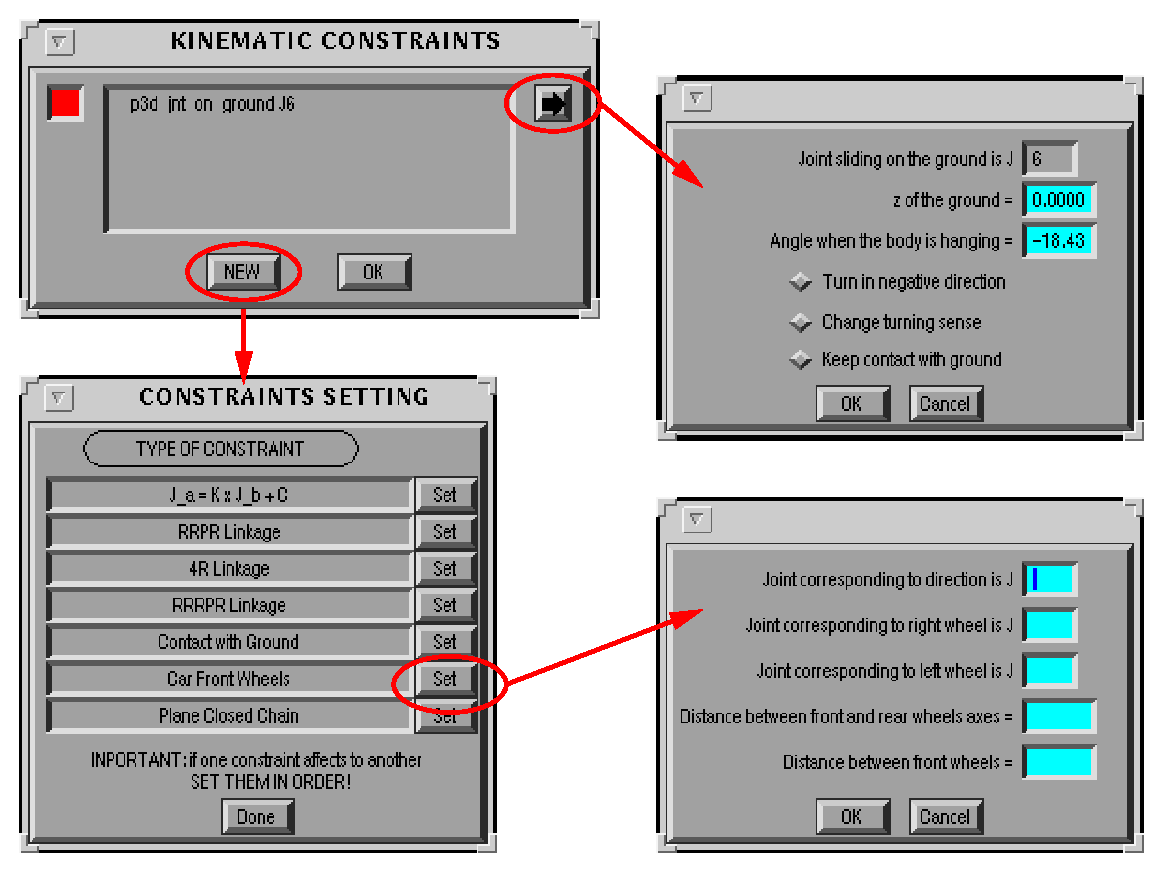
\includegraphics[width=14.0cm]{FIG/Constraint/jogwins.eps}
\end{center}
\caption{\label{fig:jogwins} Kinematic constraints window, kinematic
  constraints setting window, window containing the parameters of a
  constraint and setting window of a constraint.}
\end{figure}
 

\section{Implementation}

When a kinematic constraint is set, its data structure is
generated. This data structure contains all the necessary information
for the treatment of the constraint. The representation in C language
of this structure is:
{\tt
\begin{tabbing}
>>>>>>>>>>>>\=>>\=>>>>>>>>>>>> \= \kill
\>typedef struct cntrt \{ \\ 
\>\>  int       \> num;\\
\>\>  char      \> namecntrt[40];\\
\>\>  int       \> active;\\
\>\>  int       \> (*fct\_cntrt)(struct cntrt *ct);\\
\>\>  int       \> nactjnts, npasjnts;\\
\>\>  int       \> ndval, nival;\\
\>\>  int       \> actjnts[MAX\_ARGU\_CNTRT];\\
\>\>  int       \> actjnt\_state[MAX\_ARGU\_CNTRT];\\
\>\>  int       \> pasjnts[MAX\_ARGU\_CNTRT];\\
\>\>  int       \> argu\_i[MAX\_ARGU\_CNTRT];\\
\>\>  double    \> argu\_d[MAX\_ARGU\_CNTRT];\\
\>\>  int       \> col\_pairs[2][MAX\_ARGU\_CNTRT];\\
\>\>  struct cntrt \> *next\_cntrt;\\
\>\>  struct cntrt \> *prev\_cntrt;\\
\>\>  int       \> enchained\_J[MAX\_ARGU\_CNTRT];\\
\>\>  int       \> nenchained;\\
\>\>  struct cntrt \> **enchained;\\
\>\} p3d\_cntrt,*pp3d\_cntrt; \\
\end{tabbing}
}

Some of the members of this data structure have been already
named, and theirs values are directly given by the user. The rest
of them are automatically calculated in the setting function of each
constraint. In order to  allow a further comprehension about how the
implementation of the kinematic constraints is made, these variables
will be briefly explained next.
\begin{itemize}
\item[$-$] The data structure of each robot in the workspace of Move3D contains 
an array of pointers to the data structures of its kinematic
constraints. {\bf \tt num} represents the index of a constraint in this
list.
\item[$-$] {\bf \tt name} contains the name of the constraint.
\item[$-$] {\bf \tt active} is a flag to indicate the state of the constraint
 (activated/deactivated).
\item[$-$] {\bf \tt fct\_cntrt} is a pointer to the function
containing the equations to solve this constraint type.
\item[$-$] {\bf \tt nactjnts} and {\bf \tt npasjnts} are respectively the number
  of active and passive joints of the constraint.
\item[$-$] {\bf \tt ndval} and {\bf \tt nival} are respectively the
  number of real and integer constant parameters of the constraint
  that are given by the user.
\item[$-$] {\bf \tt actjnts} and {\bf \tt pasjnts} are arrays containing the indexes of 
the active and passive joints in this constraint.
\item[$-$] {\bf \tt actjnt\_state} is an array of flags for the active joints of
the constraint. A flag set to $0$ means that the corresponding joints
is involved in a previously defined constraint.
\item[$-$] {\bf \tt argu\_i} and {\bf \tt argu\_d} contain respectively integer and
real constant parameters of the kinematic constraint. Some of these
parameters are the ones introduced by the user. The rest are
automatically calculated. The kind of these calculated constants are, for
example: flags, distances between joints or values to refer angles.
\item[$-$] {\bf \tt col\_pairs} is used to stock information for the 
  deactivation of pairs of bodies for the collision checking.
\item[$-$] {\bf \tt next\_cntrt} and {\bf \tt prev\_cntrt} are
  pointers to the next and preceding constraints in the above
  mentioned list.
\item[$-$] {\bf \tt enchained\_J}, {\bf \tt nenchained} and {\bf \tt enchained} are used for 
  the treatment of {\em multi-constraints}. This concept will be
  explained later.
\end{itemize}


Two special remarks can be made at this point. These remarks ascribe
collision checking and multi-constraints.

Pairs of consecutive bodies
of a robot are deactivated for the collision checking in Move3D. This
same rule must be followed, for instance, when a kinematic chain is
closed. In this case, collisions between the pair of bodies closing the
chain have not to be tested. Deactivation of pairs affected by
kinematic constraints is carried out form the information stocked in the 
matrix {\tt col\_pairs}.

A special treatment of kinematic constraints have to be made when they
are {\em enchained}. A multi-constraint can be defined as several
kinematic constraints where active joints of some of them are passive
joints for some others. Two kinematic constraints obeying this property are
told to be enchained. An example of enchained constraints are
multi-loop closed chains. Notice that {\bf constraints to
  be enchained must be set in order}, that is to say: if an active
joint in a constraint is a passive joint in another one, this last
constraint must be defined first.


\section{New kinematic constraints}

The way how the treatment of kinematic constraints has been
implemented in Move3D allows that new constraints will be easily added
to the software. The work to do for this purpose have to be developed in the files {\bf
  FORMconstraints.c} and {\bf p3d\_constraints.c}. The first one
contains all the functions related with interface windows. If a new
constraint is wanted to be added, its related functions in this file
will be easily programmed by following the same procedure that for the
rest of constraints. The functions to be added in file {\bf
  p3d\_constraints.c} are the function for the setting of the new
constraint and the one containing its geometric constraint
equation(s). The calculations of the parameters related with the
constraint that are not going to change during the current running of Move3D
have to be made just once. These operations must be placed in the
setting function. The rest of the operations have to be made each time 
that the function with the constraint equation(s) is called, so they
must be placed inside it.

